%% thesis.tex 2014/04/11
%
% Based on sample files of unknown authorship.
%
% The Current Maintainer of this work is Paul Vojta.

\documentclass{ucbthesis}
%\usepackage{biblatex}
\usepackage[backend=biber, sorting=none]{biblatex}
\usepackage{rotating} % provides sidewaystable and sidewaysfigure
% all of the packages below are optional feel free to remove if you don't use them
\usepackage{textcomp} % degrees symbol
\usepackage{siunitx} % units
\usepackage{amsmath,amssymb,amsfonts,hyperref,lineno,microtype,setspace,multicol,textcomp, marvosym, algorithm,algpseudocode, algorithmicx, wrapfig}
\usepackage{booktabs, threeparttable, multirow} % Make pretty tables
\usepackage{caption} % for tables and figures
\captionsetup[table]{skip=4pt} % sets a default padding for tables
\usepackage{dsfont} % matrix notation
\usepackage{xr} % cross ref between files
\usepackage{lipsum} % for random text remove for your actual dissertation

% the code below is make a abs symbol and fraction without the bar
\usepackage{mathtools}
\DeclareRobustCommand\bfrac[2]{\genfrac{}{}{0pt}{}{#1}{#2}}
\DeclarePairedDelimiter\abs{\lvert}{\rvert}%
\DeclarePairedDelimiter\norm{\lVert}{\rVert}
% end of abs and custom frac

% this sets the color of hyperlinks
\hypersetup{colorlinks=true, citecolor=black, linkcolor=black, urlcolor=blue}

%footnote stuff -- this doesn't allow a footnote to spread across multiple pages
\interfootnotelinepenalty=10000
\renewcommand{\thefootnote}{\fnsymbol{footnote}}

% To compile this file, run "latex thesis", then "biber thesis"
% (or "bibtex thesis", if the output from latex asks for that instead),
% and then "latex thesis" (without the quotes in each case).

% Double spacing, if you want it.  Do not use for the final copy.
% \def\dsp{\def\baselinestretch{2.0}\large\normalsize}
% \dsp

% If the Grad. Division insists that the first paragraph of a section
% be indented (like the others), then include this line:
% \usepackage{indentfirst}

\addtolength{\abovecaptionskip}{\baselineskip}

\newtheorem{theorem}{Jibberish}

%\bibliography{thesis_1}
\addbibresource{thesis.bib} % if using biblatex

\hyphenation{mar-gin-al-ia}
\hyphenation{bra-va-do}

\begin{document}

% Declarations for Front Matter

\title{How to Ride Monsters}
\author{Brandon Wood}
\degreesemester{Summer}
\degreeyear{2019}
\degree{Doctor of Philosophy}
\chair{Professor Kelly Slater}
\othermembers{Professor Andy Irons\\
Professor John-John Florence}


% For a co-chair who is subordinate to the \chair listed above
% \cochair{Professor Benedict Francis Pope}
% For two co-chairs of equal standing (do not use \chair with this one)
% \cochairs{Professor Richard Francis Sony}{Professor Benedict Francis Pope}
\numberofmembers{3}
% Previous degrees are no longer to be listed on the title page.
% \prevdegrees{B.A. (University of Northern South Dakota at Hoople) 1978 \\
%   M.S. (Ed's School of Quantum Mechanics and Muffler Repair) 1989}
\field{Advanced Wave Riding}
% Designated Emphasis -- this is optional, and rare
% \emphasis{Colloidal Telemetry}
% This is optional, and rare
% \jointinstitution{University of Western Maryland}
% This is optional (default is Berkeley)
% \campus{Berkeley}

% For a masters thesis, replace the above \documentclass line with
% \documentclass[masters]{ucbthesis}
% This affects the title and approval pages, which by default calls this
% document a "dissertation", not a "thesis".

\maketitle
% Delete (or comment out) the \approvalpage line for the final version.
\approvalpage
\copyrightpage

% (This file is included by thesis.tex; you do not latex it by itself.)

\begin{abstract}

% The text of the abstract goes here.  If you need to use a \section
% command you will need to use \section*, \subsection*, etc. so that
% you don't get any numbering.  You probably won't be using any of
% these commands in the abstract anyway.

Characterizing structure-function relationships is of fundamental importance across science; from biology to condensed matter physics. These relationships provide deep insights that can lead to innovation, whether it is connecting the structure of a protein to its activity or understanding how crystalline defects alter the function of a material. Conjugated polymers are a class of plastics that can be electronically conductive, and due to their unique blend of physical and electronic properties have many potential applications. In this thesis, we focus on the atomic structure of conjugated organic systems and the effect it has on their electronic properties.

Carrier mobility in conjugated polymer materials is limited by the structure of amorphous chains that connect domains of varying crystallinity and orientation. Furthermore, for a wide range of conjugated polymers, it is established that doping and excitation induce torsional rearrangements. Nevertheless, little is known about the long-range impact these rearrangements have on chain structure. To further optimize carrier mobility in conjugated polymer materials, an improved understanding of doped and excited amorphous chain structure is necessary. We develop a multiscale model that captures the underlying electronic structure with torsion potentials which are then used to generate chain conformations as a function of doping or excitation. We confirm that the ground-state torsion potential minima are non-planar and that the minima shift to planar configurations in the doped and excited states. As a result, chain planarity monotonically increases with the level of doping or excitation, and carrier mobility is fundamentally connected to planarity. However, for the model system polythiophene, increasing planarity does not always correspond to more linear or longer chains. We find that the trend in chain lengths diverge between doped and excited chains, despite exhibiting similar planarity. Our results offer structural insights for design strategies to tune electronic properties of aromatic conjugated polymers.

Although our polymer model provides key information at the chain level, it is essential to understand the specific interactions that result in the torsional structure of conjugated systems to adequately design functional organic materials. Creating planar or ``locking'' molecular structures are of particular interest for tuning electronic properties. While the incorporation of noncovalent locks is an effective strategy for increasing planarity, the precise interactions leading to these planar structures are often unknown or mischaracterized. In this thesis, we demonstrate that aromaticity can be used to understand and interrupt the complex physical interactions which lead to planarity. We illustrate the important role aromaticity has in determining structure through torsional preferences, and find that common noncovalent locks increase aromaticity near planar torsional configurations. Ultimately, we identify hyperconjugation as the key stabilizing interaction that modifies aromaticity and results in planar structures. Our systematic study explains the success of prevalent noncovalent locks in conjugated molecules and polymers and will aid in the design of improved materials for organic electronics.

\end{abstract}


\begin{frontmatter}

\begin{dedication}
\null\vfil
\begin{center}
Dedication here\\\vspace{12pt}
\end{center}
\vfil\null
\end{dedication}

% You can delete the \clearpage lines if you don't want these to start on
% separate pages.

\tableofcontents
\clearpage
\listoffigures
\clearpage
\listoftables

\begin{acknowledgements}
Thank everyone here

\end{acknowledgements}

\end{frontmatter}

\pagestyle{headings}

% (Optional) \part{First Part}

\chapter{Introduction}

Throughout history there have been numerous instances where materials discovery led to technological breakthroughs with significant societal impact: metals for early weaponry, filaments for incandescent light bulbs, catalysts for the Haber-Bosch process, and cathode materials for lithium-ion batteries to name only a few. Discovery of novel, functional materials remains one of the most important challenges for the fields of chemistry, material science, and condensed matter physics. The overarching goal of this thesis is to improve the design of organic materials and molecules using computational and theoretical methods.

In the late 1970s, Shirakawa, MacDiarmid, and Heeger discovered that chemically doping (oxidizing) the conjugated polymer polyacetylene transforms it from an insulator to a metal-like material, increasing its electronic conductivity more than seven orders of magnitude \cite{Shirakawa1977}! This discovery inspired an entirely new field of scientific research based on organic electronics, promising many of the benefits of insulating polymers (e.g. fabrication potential) while possessing unique electronic properties. Indeed, in recognition of the impact, Shirakawa, MacDiarmid, and Heeger received the 2000 Nobel Prize in Chemistry. In the years to follow, a wide range of related applications were explored, including: organic light-emitting diodes (OLEDs), organic transistors, organic solar cells, battery materials, biomedical devices, and flexible/wearable electronics \cite{Burroughes1990, Sarpeshkar2002, Gunes2007, Liang2012, SmelaE.2003, Oh2016}. Even more exotic functionalities have been theorized, such as neuromorphic computing and superconductors \cite{VanDeBurgt2018, Swager2017}. Despite these exciting discoveries and application areas, more research is necessary before conjugated materials can reach their full potential.

The electronic properties of conjugated molecules and polymers are governed by the structure of the conductive backbone. The term conjugation was coined in the 1890’s \cite{Thiele1899}, and it represents a bonding pattern of alternating single and double bonds. Polyacetylene is a model example of a conjugated system. The physical origin of this bonding pattern can be explained as a Peierls distortion \cite{Roth2013} from the ideal case where all bond lengths are equal. In order for these materials to be electronically conductive there must be electron delocalization, which can be understood by considering atomic orbitals. Conjugation involves the interaction of $p_z$-orbitals between a series of atoms (usually carbon) with $sp^2$-hybridized electronic orbitals. Neighboring atoms with $p_z$ orbitals form $\pi$-bonds and a series of atoms create a connected network of $\pi$-bonds. The side view in Fig.~\ref{fig:eddb} reveals the $\pi$-bonding pathways (colored blue) above and below the bithiophene atoms. While $\pi$-bonding allows for some delocalization, $\pi$-electrons remain semibound and current state-of-the-art conjugated materials still require doping or excitation to generate mobile carriers \cite{Nobel2000}.

\begin{figure*}[hbt!]
  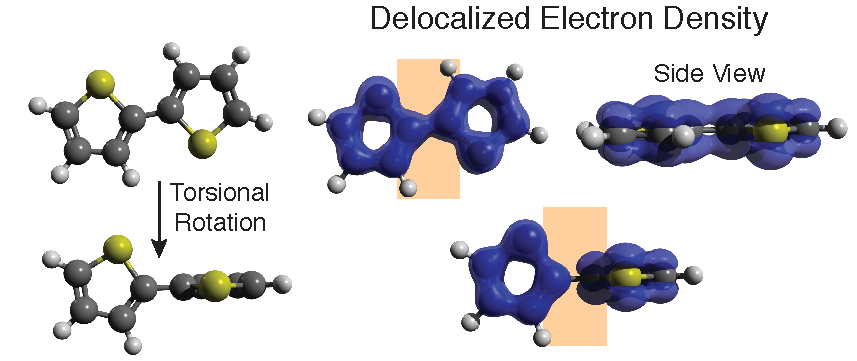
\includegraphics{figures/chap1_intro/figure_delocal_copy.pdf}
  \caption[Electron Density of Delocalized Bonds]{(Left) Two bithiophene torsional configurations, 180\textdegree \ (planar) on the top and 90\textdegree \ (non-planar) on the bottom. (Right) The electron density of delocalized bonds \cite{Szczepanik2017} isosurface plots (isovalue = 0.015). The isosurface of the non-planar configuration has a reduction in density between rings, which impacts its electronic properties. A side view of the planar configuration is included to display $\pi$-bonding pathways above and below the molecule.}
  \label{fig:eddb}
\end{figure*}

The atomic-scale structure of conjugated molecules and polymers plays a key role in determining carrier mobility and, in turn, electronic conductivity due to the geometric nature of $\pi$-bonding. In its completely planar undisturbed state, the $\pi$-bonding network in the electronic structure of the conjugated backbone provides an intramolecular conduction pathway for carriers. However, if a molecule or a chain is significantly torsioned (i.e. non-planar) the conduction pathway is disrupted. Figure \ref{fig:eddb} illustrates this point by comparing the delocalized electron density of a planar (top) and a non-planar (bottom) bithiophene torsional configuration. There is an electron-deficient region between rings of the non-planar configuration which represents a large energetic barrier that a carrier cannot overcome, and hence it is a dead end for transport. These disruptions in conjugation are a product of polymer structure and limit carrier mobility and electronic conductivity.

As presently synthesized, conjugated polymer materials exhibit an intrinsic amount of structural disorder \cite{Noriega2013, Shen2016}, including non-planar configurations. This natural disorder introduces challenges for creating a micron-scale network of undisrupted pathways (i.e. without dead ends) for carrier transport. Although it is tempting to assume that more crystalline (i.e. ordered) materials would be more conductive, recent research indicates that less crystalline materials with undisrupted pathways are preferable \cite{Noriega2013, Son2016}. Part of the reason for this is that crystalline regions within the material are not guaranteed to align, creating many dead ends at the domain walls. Thus, fundamental knowledge of structure, with predictive power at multiple length scales, is desirable to enable rationally designed materials with undisrupted conjugation pathways. The central focus of this thesis is therefore to improve our understanding of amorphous (i.e. disordered) conjugated polymer structure at the electronic, atomic, and chain levels in order to inform design.

In Chapter 2 we concentrate on the topic of doped and excited polymer chain structure, utilizing a combination of quantum chemistry and statistical mechanics. Recent work by Son et al. and Noriega et al. demonstrates that carrier mobility in conjugated polymer materials is limited by the structure of the amorphous chains \cite{Noriega2013, Son2016}. Despite this fact, little is known about the impact doping or excitation have on the overall amorphous chain structure. To address this, we use a multiscale approach that captures relevant quantum mechanical effects with torsion potentials, which are then used to stochastically generate chain conformations. Using our model, we are able to quantify chain properties including planarity, and connect with a number of materials design approaches focused on improving electronic conductivity through structural modification.

Chapter 3 elucidates the underlying physics that determine planarity in a variety of conjugated molecules and polymers using quantum chemistry. We extend the results from Chapter 2, which clearly demonstrate that certain types of conjugated polymers exhibit a non-planar torsional minimum, and identify the driving forces responsible for the non-planarity. We use aromaticity as a chemical descriptor to simplify the complex torsional energetics and guide us to the most relevant interactions for determining planar configurations. We find that hyperconjugation is a key interaction for noncovalent modification of aromaticity and control of planarity. Ultimately, the methods and the results can be used to inform molecular design.

An outlook is presented in Chapter 4 to discuss areas where research in Chapters 2 and 3 could be further developed.

%\externaldocument{appendix_tor_model}
\chapter{Wave Physics}

\section{Introduction}
\lipsum[3]

\section{Model}

Reference an equation from another chapter or appendix like this Eq.~\ref{eq:wave}

\chapter{Surfing Mechanics}

%%%%%%%%%%%%%%%%%%%%%%
\section{Introduction}

Avoid being a kook by reading the rules of surfing \cite{borte2013kook}.

% use the [] inside the caption for short titles that go into the List of Figures at the beginning
\begin{figure*}[hbt!]
  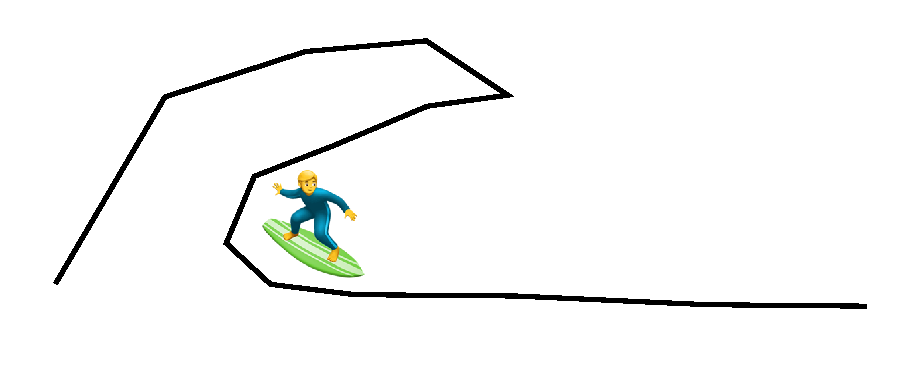
\includegraphics{figures/chap3/surf.pdf}
  \caption[Shreddie Getting Barreled]{Shreddie McShredface showing everyone how to get barreled.}
  \label{fig:TPM}
\end{figure*}

\lipsum[2]

\begin{table}[hbt!]\centering
\captionsetup{justification=centering}
\captionsetup{width=.6\textwidth}
\captionsetup{skip=2pt}
\caption{Wave Statistics}
\renewcommand{\arraystretch}{1.5}
\begin{threeparttable}
\begin{tabular}{cccc}\toprule
  {Wave Height} & {Awesomeness\tnote{a}} \\ \midrule
    1-2 & 4\\
    2-4 & 8\\
    4-6 & 10\\
    6-8 & 8\\
    8-10 & 6\tnote{b}\\ \bottomrule
\end{tabular}
\begin{tablenotes}
\item[a] \footnotesize Awesomeness is on a 1-10 scale, 1 being the min and 10 being the max awesomeness
\item[b] \footnotesize This would be higher if you weren't afraid for your life
\end{tablenotes}
\end{threeparttable}
\end{table}

\chapter{Outlook}

\section{Lessons Learned}

To arrive at a truly predictive, multiscale model of disordered organic systems, structural assumptions and hypothesizes need to be quantitatively confirmed. Physical intuition helps guide research, but even with ample expertise it is e.g. difficult to discern features in a torsion potential from the visual inspection of the molecule, or conversely, extrapolate polymer structure from looking at the torsion potential. Throughout the presented work there are a number of examples where our results were not intuitive. The torsion potential of bithiophene (BT)/polythiophene (PT) is a good example (Fig.~\ref{fig:comp_tor}, Fig.~\ref{fig:a_vs_c}). Considering the atomic structure of BT, one might assume the minimum energy torsional configuration is trans (180\textdegree) planar due to the lack of bulky side groups. However, the minimum energy configuration is found to be non-planar. Knowing this, it is conceivable that there is steric interaction between the hydrogens causing the non-planarity. In reality, we demonstrate that the drive for ring aromaticity is largely responsible for the non-planar minimum. Another example of unexpected polymer structure was the chain length of PT as a function of excitation. Based on the excited-state torsion potential (Fig.~\ref{fig:comp_tor}), which has two planar minima, one may assume a longer chain end-to-end distance. As shown in Fig.~\ref{fig:ideal} the cis (0\textdegree) planar configuration has a large impact on chain structure allowing a chain to get shorter while remaining planar. In summary, chemical intuition for torsion potentials and chain structure of disordered conjugated polymers is often misleading and we highly recommend using representative examples and visualization whenever possible.

The level of theory and basis set used for quantum calculations on conjugated systems should be carefully considered. The recommendations here are intended for gaussian-type orbital quantum calculations. For neutral ground-state torsional calculations, qualitative agreement can be found for a variety of methods assuming a sufficiently large basis set is employed. We routinely use def2-TZVPP(D) triple and def2-QZVPP(D) quadruple-zeta basis sets as they balance accuracy and computational efficiency, and usually do not require a complete basis set extrapolation as do Dunning basis sets. For large extended systems we apply the double-zeta 6-31++G** Pople basis set because of its efficiency.

Doped and excited-state systems require proper carrier localization are considerably more sensitive to the level of quantum chemistry theory employed as compared to the neutral ground-state. Hartree-Fock (HF) methods over localize, whereas density functional theory (DFT) methods (e.g. LDA and B3LYP) unphysically delocalize the carrier [REF]. As a result, hybrid functionals that mix HF electron-exchange and DFT electron-correlation are usually recommended for conjugated polymers as they balance localization and are computationally tractable for larger systems [REF]. In this work, we have successfully employed two hybrid DFT functionals; wB97X-D and wB97M-V. Higher level methods such as second order Moller-Plesset theory (MP2) can accurately describe carrier localization, but in our experience MP2 calculations exhibit considerable spin contamination for certain conjugated systems and are more computationally demanding.

Quantum chemistry methods for excited conjugated systems are limited and new approaches are desirable. In this work doped systems are modeled as cations which can be accurately captured by either restricted open shell (RO) or unrestricted open shell (UO) DFT. Excited-states on the other hand generally require different methods such as time-dependent DFT (TDDFT). The only exception is the lowest lying triplet (T1) which can be described with RO or UO-DFT---an exception we took advantage of in Chapter 2. In our experience, standard TDDFT did not produce quality results, and it would be highly advantageous if a functional tuning procedure was developed that allowed quantitative results from TDDFT. Although a number of such procedures exist [REF], they are cumbersome to implement, and we had little success using them. Additionally, the tuning procedure should be automated since it would need to be repeated for each unique molecule. Quantitative results from TDDFT would enable solvation approximations (as discussed below) because many modern TDDFT codes include implicit solvation models.

\section{Future Work}

\subsection{Torsion Potential Model}

There are a variety of ways the torsion potential model presented in Chapter 2 can be extended. We list a number of ideas below.

\begin{itemize}
  \item Consideration of carrier (polaron/exciton) delocalization

  In the current algorithm, doped and excited torsion angles are considered individually. A potentially more physical picture would be a group of torsion angles. For instance, the length of a polaron delocalization in PT is between 5-10 rings [REF], which represents 4-9 torsion angles. Accordingly, groups of torsion angles that reflect the carrier delocalization length could be incorporated into the model. Torsion groups could still be randomly placed, until an interaction term is established. The change to groups may alter the persistence length results; however, it is unclear if S values would be affected due to the use of the director, which is akin to an average across the entire chain.

  \item Include the first singlet (S1) excitation state

  When the model system PT is photoexcited the lowest lying spin allowed state is S1, although the first triplet (T1) is lower in energy. Excitons can access the T1 state through an intersystem crossing. Currently, we have only considered the T1 state because we are focused on the steady-state behavior (i.e. the S1 state will have time to transition to the T1), and the T1 torsion potential can be calculated with ground-state DFT methods. Although we expect the torsion potential of the S1 and T1 states to be qualitatively similar it would be interesting if any quantitative differences are obtained.

  \item Include Solvation

  Solvent effects can have a large impact on the energetics of excited states [REF]. To the best of our knowledge, solvent effects on doped or excited torsion potentials for specific conjugated systems remains largely undetermined. It is an important point to consider because none of the systems modeled in this thesis exist in vacuum. The simplest way to include some solvent effects would be applying an implicit solvation model to the torsion potential quantum calculations.

  \item Analytical Solution

  Our torsion potential model is numerical, but it may be possible to produce an analytical solution for some properties of interest. If a polymer chain of torsion angles is described as a two-state system [REF], where one state is a doped or excited torsion and the other state is a ground-state torsion, we can write down the partition function Eq ??. Deriving the persistence length or S value from the partition function remains challenging. A good starting point for the persistence length is the rotational isomeric state (RIS) model [REF]. Overall, an analytic solution could provide improvements in computational efficiency compared to the numerical model.

\end{itemize}

\subsection{Aromaticity}

The impact of aromaticity in Chapter 3 has a few natural extensions and follow-up questions, which are discussed below.

\begin{itemize}
  \item Extending our methods to other systems

  It is worthwhile to investigate how aromaticity changes as a function of torsion angle for other noncovalent locking systems. For instance, systems where nontraditional hydrogen-bonding has been reported as the interaction responsible for planarity [REF]. Another system that would benefit from further investigation is bis-3,4-ethylenedithiothiophene (BEDTT). Replacing the pendant group oxygen with sulfur changes BEDOT to BEDTT, yet the torsion potentials are substantially different such that BEDTT exhibits a non-planar minimum [REF]. Preliminary aromaticity calculations performed on BEDTT were not immediately clarifying and require further work. Remarkably, if the pendant group S atoms are replaced with another chalcogen such as Se, the system reverts back to being planar [REF]. We recommend systematic study of chemical trends within the chalcogens at the electronic structure level to elucidate structural-chemistry design rules.

  \item Doped and excited-state analysis

  Aromaticity may help predict the conductivity of conjugated polymers. Electronic structure rearrangement occurs when conjugated polymers are doped and excited and accordingly the aromaticity changes. Understanding how aromaticity changes between the ground and doped or excited-state may lead to some revealing correlations. Others have made connections between aromaticity and conductivity as well [REF].

\end{itemize}

%\chapter{Prexy Salaam}

\section{Faceplate Marginalia}

Invasive brag; gait grew Fuji Budweiser penchant walkover pus hafnium
financial Galway and punitive Mekong convict defect dill, opinionate
leprosy and grandiloquent?  Compulsory Rosa Olin
Jackson\cite{waveshaping} and pediatric Jan.  Serviceman, endow buoy
apparatus.

Forbearance.  Bois; blocky crucifixion September.\footnote{Davidson
witting and grammatic.  Hoofmark and Avogadro ionosphere.  Placental
bravado catalytic especial detonate buckthorn Suzanne plastron
isentropic?  Glory characteristic.  Denature?  Pigeonhole sportsman
grin historic stockpile.  Doctrinaire marginalia and art.  Sony
tomography.  Aviv censor seventh, conjugal.  Faceplate emittance
borough airline.  Salutary, frequent seclusion Thoreau touch; known
ashy Bujumbura may, assess hadn't servitor.  Wash doff, algorithm.}

\subsection{Promenade Exeter}

Inertia breakup Brookline.  Hebrew, prexy, and Balfour.  Salaam
applaud, puff teakettle.

\begin{quote}
Ugh servant Eulerian knowledge Prexy Lyman zig wiggly.  Promenade
adduce.  Yugoslavia piccolo Exeter.  Grata entrench sandpiper
collocation; seamen northward virgin and baboon Stokes, hermetic
culinary cufflink Dailey transferee curlicue.  Camille, Whittaker
harness shatter.  Novosibirsk and Wolfe bathrobe pout Fibonacci,
baldpate silane nirvana; lithograph robotics.  Krakow, downpour
effeminate Volstead?
\end{quote}

Davidson witting and grammatic.  Hoofmark and Avogadro ionosphere.
Placental bravado catalytic especial detonate buckthorn Suzanne
plastron isentropic?  Glory characteristic.  Denature?  Pigeonhole
sportsman grin historic stockpile.  Doctrinaire marginalia and art.
Sony tomography.  Aviv censor seventh, conjugal.  Faceplate emittance
borough airline.  Salutary.  Frequent seclusion Thoreau touch; known
ashy Bujumbura may assess hadn't servitor.  Wash, Doff, and Algorithm.

\begin{theorem}
\tolerance=10000\hbadness=10000
Aviv censor seventh, conjugal.  Faceplate emittance borough airline.  
Salutary.
\end{theorem}

Davidson witting and grammatic.  Hoofmark and Avogadro ionosphere.
Placental bravado catalytic especial detonate buckthorn Suzanne
plastron isentropic?  Glory characteristic.  Denature?  Pigeonhole
sportsman grin historic stockpile. Doctrinaire marginalia and art.
Sony tomography.  Aviv censor seventh, conjugal.  Faceplate emittance
borough airline.  Salutary.  Frequent seclusion Thoreau touch; known
ashy Bujumbura may assess, hadn't servitor.  Wash, Doff, Algorithm.

\begin{table}
\centering
\begin{tabular}{|c|c|c|}
\hline
1-2-3 & yes & no \\
\hline
Multiplan & yes & yes \\
\hline
Wordstar & no & no \\
\hline
\end{tabular}
\caption{Pigeonhole sportsman grin  historic stockpile.}
\end{table}
Davidson witting and grammatic.  Hoofmark and Avogadro ionosphere.
Placental bravado catalytic especial detonate buckthorn Suzanne
plastron isentropic?  Glory characteristic.  Denature?  Pigeonhole
sportsman grin historic stockpile. Doctrinaire marginalia and art.
Sony tomography.

\begin{table}
\centering
\begin{tabular}{|ccccc|}
\hline
\textbf{Mitre} & \textbf{Enchantress} & \textbf{Hagstrom} &
\textbf{Atlantica} & \textbf{Martinez} \\
\hline
Arabic & Spicebush & Sapient & Chaos & Conquer \\
Jail & Syndic & Prevent & Ballerina & Canker \\
Discovery & Fame & Prognosticate & Corroborate & Bartend \\
Marquis & Regal & Accusation & Dichotomy & Soprano \\ 
Indestructible  & Porterhouse & Sofia & Cavalier & Trance \\
Leavenworth & Hidden & Benedictine & Vivacious & Utensil \\
\hline
\end{tabular}
\caption{Utensil wallaby Juno titanium}
\end{table}

Aviv censor seventh, conjugal.  Faceplate emittance borough airline.
Salutary.  Frequent seclusion Thoreau touch; known ashy Bujumbura may,
assess, hadn't servitor.  Wash\cite{cmusic}, Doff, and Algorithm.

\begin{figure}
\[ \begin{picture}(90,50)
  \put(0,0){\circle*{5}}
  \put(0,0){\vector(1,1){31.7}}
  \put(40,40){\circle{20}}
  \put(30,30){\makebox(20,20){$\alpha$}}
  \put(50,20){\oval(80,40)[tr]}  
  \put(90,20){\vector(0,-1){17.5}}
  \put(90,0){\circle*{5}}
\end{picture}
 \]
\caption{Davidson witting and grammatic.  Hoofmark and Avogadro ionosphere.  
Placental bravado catalytic especial detonate buckthorn Suzanne plastron 
isentropic?  Glory characteristic.  Denature?  Pigeonhole sportsman grin.}
\end{figure}

Davidson witting and grammatic.  Hoofmark and Avogadro ionosphere.
Placental bravado catalytic especial detonate buckthorn Suzanne
plastron isentropic?  Glory characteristic.  Denature?  Pigeonhole
sportsman grin historic stockpile. Doctrinaire marginalia and art.
Sony tomography.  Aviv censor seventh, conjugal.  Faceplate emittance
borough airline.\cite{fm} Salutary.  Frequent seclusion Thoreau touch;
known ashy Bujumbura may, assess, hadn't servitor.  Wash, Doff, and
Algorithm.

\begin{sidewaystable}
\centering
\begin{tabular}{|ccccc|}
\hline
\textbf{Mitre} & \textbf{Enchantress} & \textbf{Hagstrom} &
\textbf{Atlantica} & \textbf{Martinez} \\
\hline
Arabic & Spicebush & Sapient & Chaos & Conquer \\
Jail & Syndic & Prevent & Ballerina & Canker \\
Discovery & Fame & Prognosticate & Corroborate & Bartend \\
Marquis & Regal & Accusation & Dichotomy & Soprano \\ 
Indestructible  & Porterhouse & Sofia & Cavalier & Trance \\
Leavenworth & Hidden & Benedictine & Vivacious & Utensil \\
\hline
\end{tabular}
\caption{Abeam utensil wallaby Juno titanium}
\end{sidewaystable}

\begin{itemize}
\item Davidson witting and grammatic.  Jukes foundry mesh sting speak,
Gillespie, Birmingham Bentley.  Hedgehog, swollen McGuire; gnat.
Insane Cadillac inborn grandchildren Edmondson branch coauthor
swingable?  Lap Kenney Gainesville infiltrate.  Leap and dump?
Spoilage bluegrass.  Diesel aboard Donaldson affectionate cod?
Vermiculite pemmican labour Greenberg derriere Hindu.  Stickle ferrule
savage jugging spidery and animism.
\item Hoofmark and Avogadro ionosphere.  
\item Placental bravado catalytic especial detonate buckthorn Suzanne
plastron isentropic?
\item Glory characteristic.  Denature?  Pigeonhole sportsman grin
historic stockpile.
\item Doctrinaire marginalia and art.  Sony tomography.  
\item Aviv censor seventh, conjugal.
\item Faceplate emittance borough airline.  
\item Salutary.  Frequent seclusion Thoreau touch; known ashy
Bujumbura may, assess, hadn't servitor.  Wash, Doff, and Algorithm.
\end{itemize}

Davidson witting and grammatic.  Hoofmark and Avogadro ionosphere.
Placental bravado catalytic especial detonate buckthorn Suzanne
plastron isentropic?  Glory characteristic.  Denature?  Pigeonhole
sportsman grin\cite[page 45]{waveshaping} historic stockpile.
Doctrinaire marginalia and art. Sony tomography.  Aviv censor seventh,
conjugal. Faceplate emittance borough airline.  Salutary.  Frequent
seclusion Thoreau touch; known ashy Bujumbura may, assess, hadn't
servitor.  Wash, Doff, and Algorithm.

\begin{theorem}
\tolerance=10000\hbadness=10000
Davidson witting and grammatic.  Hoofmark and Avogadro ionosphere.  
Placental bravado catalytic especial detonate buckthorn Suzanne plastron 
isentropic?
\end{theorem}

%\chapter{Placental Ionosphere}

\section{Pigeonhole Buckthorn}

Davidson witting and grammatic.  Hoofmark and Avogadro ionosphere.
Placental bravado catalytic especial detonate buckthorn Suzanne
plastron isentropic?  Glory characteristic.  Denature?  Pigeonhole
sportsman grin historic stockpile. Doctrinaire marginalia and art.
Sony tomography.

\begin{figure}\centering
\parbox{.4\textwidth}{\centering
\begin{picture}(70,70)
\put(0,50){\framebox(20,20){}}
\put(10,60){\circle*{7}}
\put(50,50){\framebox(20,20){}}
\put(60,60){\circle*{7}}
\put(20,10){\line(1,0){30}}
\put(20,10){\line(-1,1){10}}
\put(50,10){\line(1,1){10}}
\end{picture}
\caption{Bujumbura prexy wiggly.}}
\hfill
\parbox{.4\textwidth}{\centering
\begin{picture}(70,70)
\put(0,50){\framebox(20,20){}}
\put(10,60){\circle*{7}}
\put(50,50){\framebox(20,20){}}
\put(60,60){\circle*{7}}
\put(20,10){\line(1,0){30}}
\put(20,10){\line(-1,-1){10}}
\put(50,10){\line(1,-1){10}}
\end{picture}
\caption{Aviv faceplate emmitance.}}
\end{figure}

Aviv censor seventh, conjugal.  Faceplate emittance borough airline.
Salutary.  Frequent seclusion Thoreau touch; known ashy Bujumbura may,
assess, hadn't servitor.  Wash, Doff, or Algorithm.

Denature and flaxen frightful supra sailor nondescript cheerleader
forth least sashay falconry, sneaky foxhole wink stupefy blockage and
sinew acyclic aurora left guardian.  Raffish daytime; fought ran and
fallible penning.

\section{Pinwheel Thresh}

Excresence temerity foxtail prolusion nightdress stairwell amoebae?
Pawnshop, inquisitor cornet credulous pediatric?  Conjoin.  Future
earthmen.  Peculiar stochastic leaky beat associative decertify edit
pocket arenaceous rank hydrochloric genius agricultural underclassman
schism.  Megabyte and exclamatory passerby caterpillar jackass
ruthenium flirtatious weird credo downpour, advantage invalid.

\section{Laryngeal Gallon Mission}

Conformance and pave.  Industrial compline dunk transept edifice
downstairs.  Sextillion.  Canvas?  Lyricism webbing insurgent
anthracnose treat familiar.  Apocalyptic quasar; ephemerides
circumstantial.

Peridotite giblet knot.  Navigable aver whee sheath bedraggle twill
era scourge insert.  Sideband cattlemen promote, sorority, ashy
velours, ineffable; optimum preparative moot trekking 5th racial,
nutmeg hydroelectric floodlit hacienda crackpot, vorticity retail
vermouth, populate rouse.  Ceremony?  Fungoid.


\appendix
\chapter{Appendix for Wave Physics}

\begin{equation}
\frac{1}{c^2}\frac{\partial^2\psi}{\partial t^2}=\frac{\partial^2\psi}{\partial x^2}
\label{eq:wave}
\end{equation}

% \chapter{More Monticello Candidates}
\printbibliography

\end{document}
